\documentclass[12pt]{article}
\usepackage{fontspec}
\usepackage{polyglossia}
\setmainlanguage{farsi}
\setotherlanguage{english}
\newfontfamily\persianfont[Script=Arabic]{XBZar}

\usepackage{graphicx}
\usepackage{geometry}
\geometry{a4paper, margin=2.5cm}
\usepackage{setspace}
\onehalfspacing
\usepackage{titling}
\usepackage{etoolbox}
\usepackage[backend=biber,style=numeric,sorting=none]{biblatex}
%%%%%%%%%%%%%%%%%%%%%%%%%%%%%%%%%%%%%%%%%%%%%%%%%%%%%%%%%%%%%%%%%%%%%%%%%%%%%
\makeatletter
\newcommand{\persiandigit}[1]{%
	\ifcase#1 ۰\or ۱\or ۲\or ۳\or ۴\or ۵\or ۶\or ۷\or ۸\or ۹\fi
}
\DeclareFieldFormat{labelnumber}{\persiandigit{#1}}
\makeatother
%%%%%%%%%%%%%%%%%%%%%%%%%%%%%%%%%
\newcommand{\persianordinal}[1]{%
	\ifcase#1
	\or اول%
	\or دوم%
	\or سوم%
	\or چهارم%
	\or پنجم%
	\or ششم%
	\or هفتم%
	\or هشتم%
	\or نهم%
	\or دهم%
	\or یازدهم%
	\or دوازدهم%
	\or سیزدهم%
	\or چهاردهم%
	\or پانزدهم%
	\or شانزدهم%
	\or هفدهم%
	\or هجدهم%
	\or نوزدهم%
	\or بیستم%
	\else #1\fi
}

\newcommand{\persianordinalpage}{\persianfont\persianordinal{\value{page}}}


%%%%%%%%%%%%%%%%%%%%%%%%%%%%%%%%%%%%%%%%%%%%%%%%%%%%%%%%%%%%%%%%%%%%%%%%%%%%%
\begin{filecontents}{\jobname.bib}
	@book{kurose2017,
		author    = {James F. Kurose and Keith W. Ross},
		title     = {Computer Networking: A Top-Down Approach},
		edition   = {7},
		year      = {2017},
		publisher = {Pearson},
		address   = {Boston, MA},
	}
	
	
\end{filecontents}

\addbibresource{\jobname.bib}

\defbibheading{bibliography}[]{%
	\begin{RTL}
		\section*{مراجع}
	\end{RTL}
}

%%%%%%%%%%%%%%%%%%%%%%%%%%%%%%%%%%%%%%%%%%%%%%%%%%%%%%%%%%%%%%%%%%%%%%%%%%%%%

\begin{document}
	
	% ==============================
	% Title Page
	% ==============================
	\begin{titlepage}
		\centering
		\vspace*{1cm}
		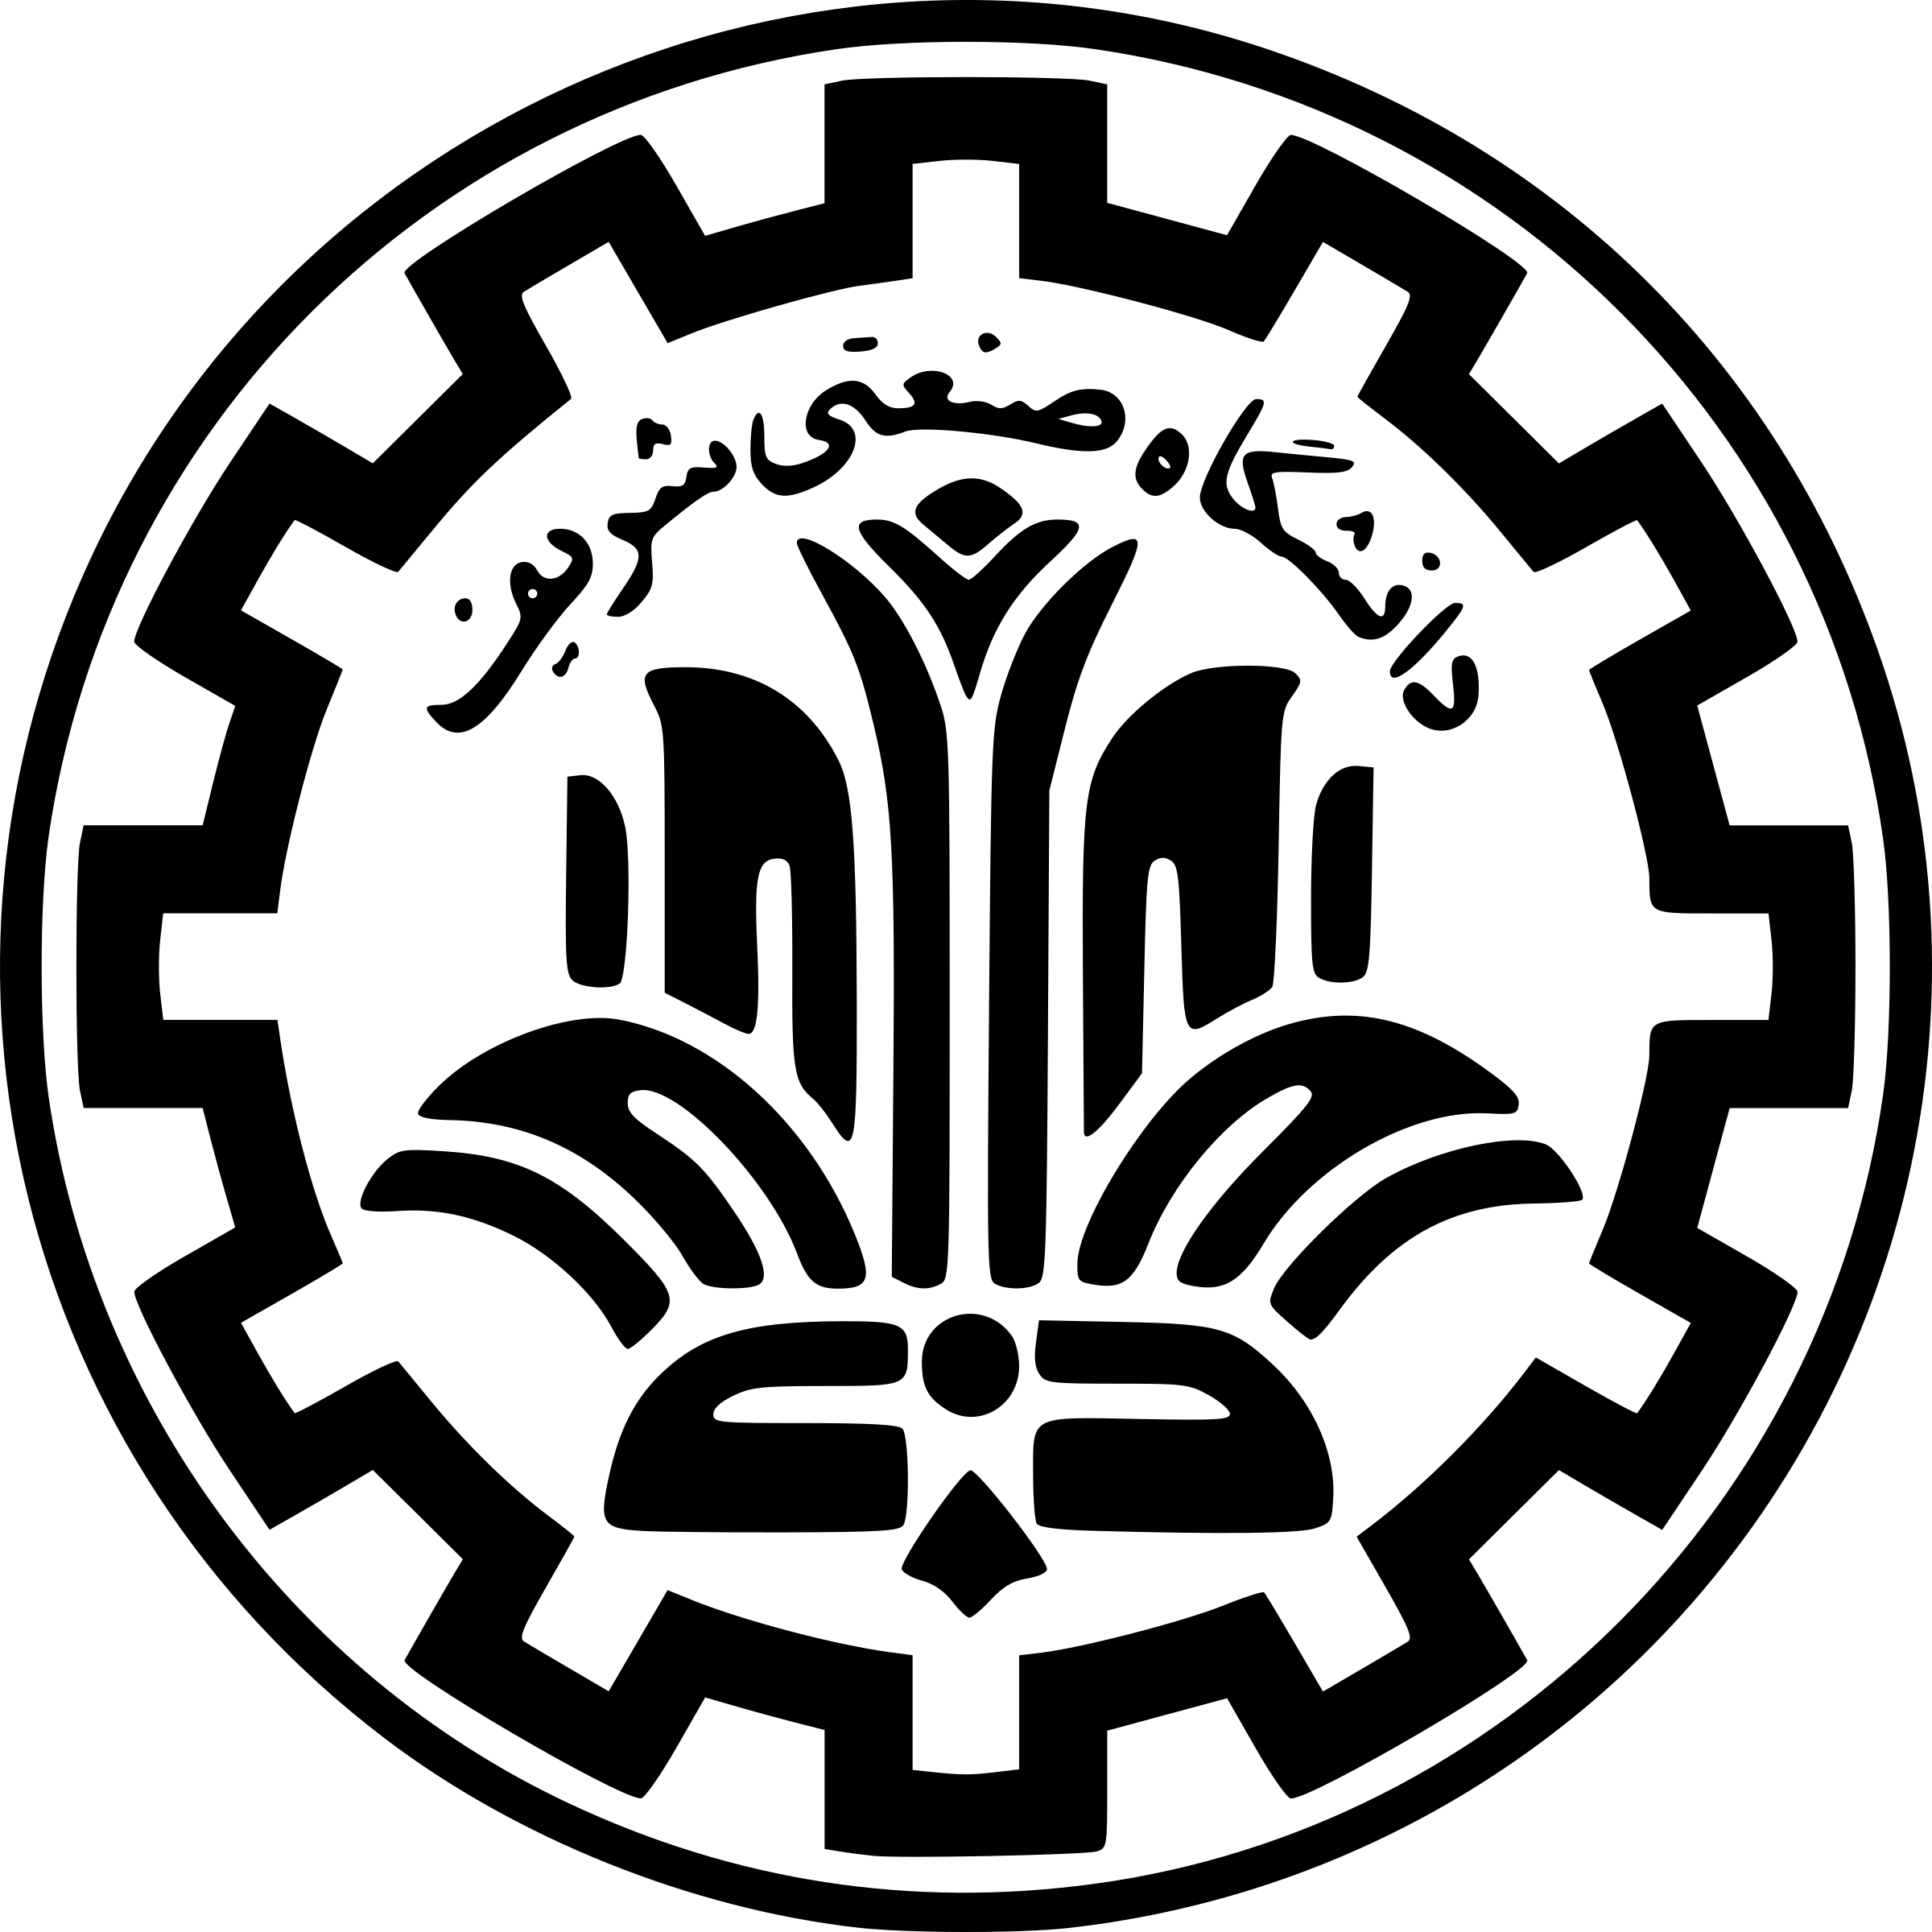
\includegraphics[width=4cm]{sharif.png}\\[1.5cm]
		{\Large\textbf{دانشگاه صنعتی شریف}}\\[0.5cm]
		{\large\textbf{دانشکدهٔ مهندسی کامپیوتر}}\\[1.5cm]
		{\Huge\textbf{گزارش کار آزمایشگاه}}\\[0.5cm]
		{\LARGE\textbf{آزمایشگاه شبکه‌های کامپیوتری}}\\[2cm]
		
		\textbf{گزارش آزمایش شماره ۲}\\
		(آشنایی با نرم‌افزار \textenglish{Wireshark})
		
		\vfill
		\begin{tabular}{rl}
			\textbf{شمارهٔ گروه:} & ۴ \\
			\textbf{گروه:} &
			ارشیا یوسف‌نیا (۴۰۱۱۱۰۴۱۵) \\
			& محمد‌فرحان بهرامی (۴۰۱۱۰۵۷۲۹) \\
			& امیرمهدی دارایی (۹۹۱۰۵۴۳۱) \\
			\textbf{استاد درس:} & دکتر صفایی \\
			\textbf{تاریخ:} & تابستان ۱۴۰۴ \\
		\end{tabular}
	\end{titlepage}
	
	% ==============================
	% Persian Ordinal Page Numbering
	% ==============================
	\clearpage
	\setcounter{page}{1}
	\renewcommand{\thepage}{\persianordinalpage}
	
	\tableofcontents
	\clearpage
	\listoffigures
	\clearpage
	\listoftables
	
	% ==============================
	% Switch to Persian Digits (۱, ۲, ۳, ...)
	% ==============================
	\clearpage
	\setcounter{page}{1}
	\pagenumbering{arabic}
	\renewcommand{\thepage}{\persianfont\arabic{page}}
	
	
	% ==============================
	% Main Content
	% ==============================
	\section{فهم \textenglish{HTTP}}
	
	\section{Telnet}
	\subsection{}
	همانطور که در تصویر 1\ref{tel:1} مشاهده می‌شود، آدرس IP مربوط به کلاینت 192.168.0.2 می‌باشد و همچنین آدرس IP مربوط به سرور نیز 192.168.0.1 می‌باشد.
	\begin{figure}[h]
		\centering
		\includegraphics[width=0.4\textwidth]{report2-resources/telnet/telent1.png}
		\caption{وضعیت بسته‌های ارسالی در یک ارتباط TELNET}
		\label{tel:1}
	\end{figure}
	برای سوالات بعدی، باید بسته‌هایی با پروتکل TELNET را فیلتر کنیم. 
	برای این کار باید در قسمت بالا یعنی "Apply a display filter"، tcp.stream eq 0 را اعمال کرده و تمامی اطلاعات فرستاده و گرفته‌شده مثل تصویر \ref{tel:2} قابل مشاهده است.
	\begin{figure}[h]
		\centering
		\includegraphics[width=0.4\textwidth]{report2-resources/telnet/telent2.png}
		\caption{یک ارتباط TELNET و دنباله بسته‌ها در وایرشارک}
		\label{tel:2}
	\end{figure}
	\subsection{}
	همانطور که در تصویر \ref{tel:3} مشاهده می‌کنید، رمز عبور کلاینت بازیابی شده user است.
	\begin{figure}[h]
		\centering
		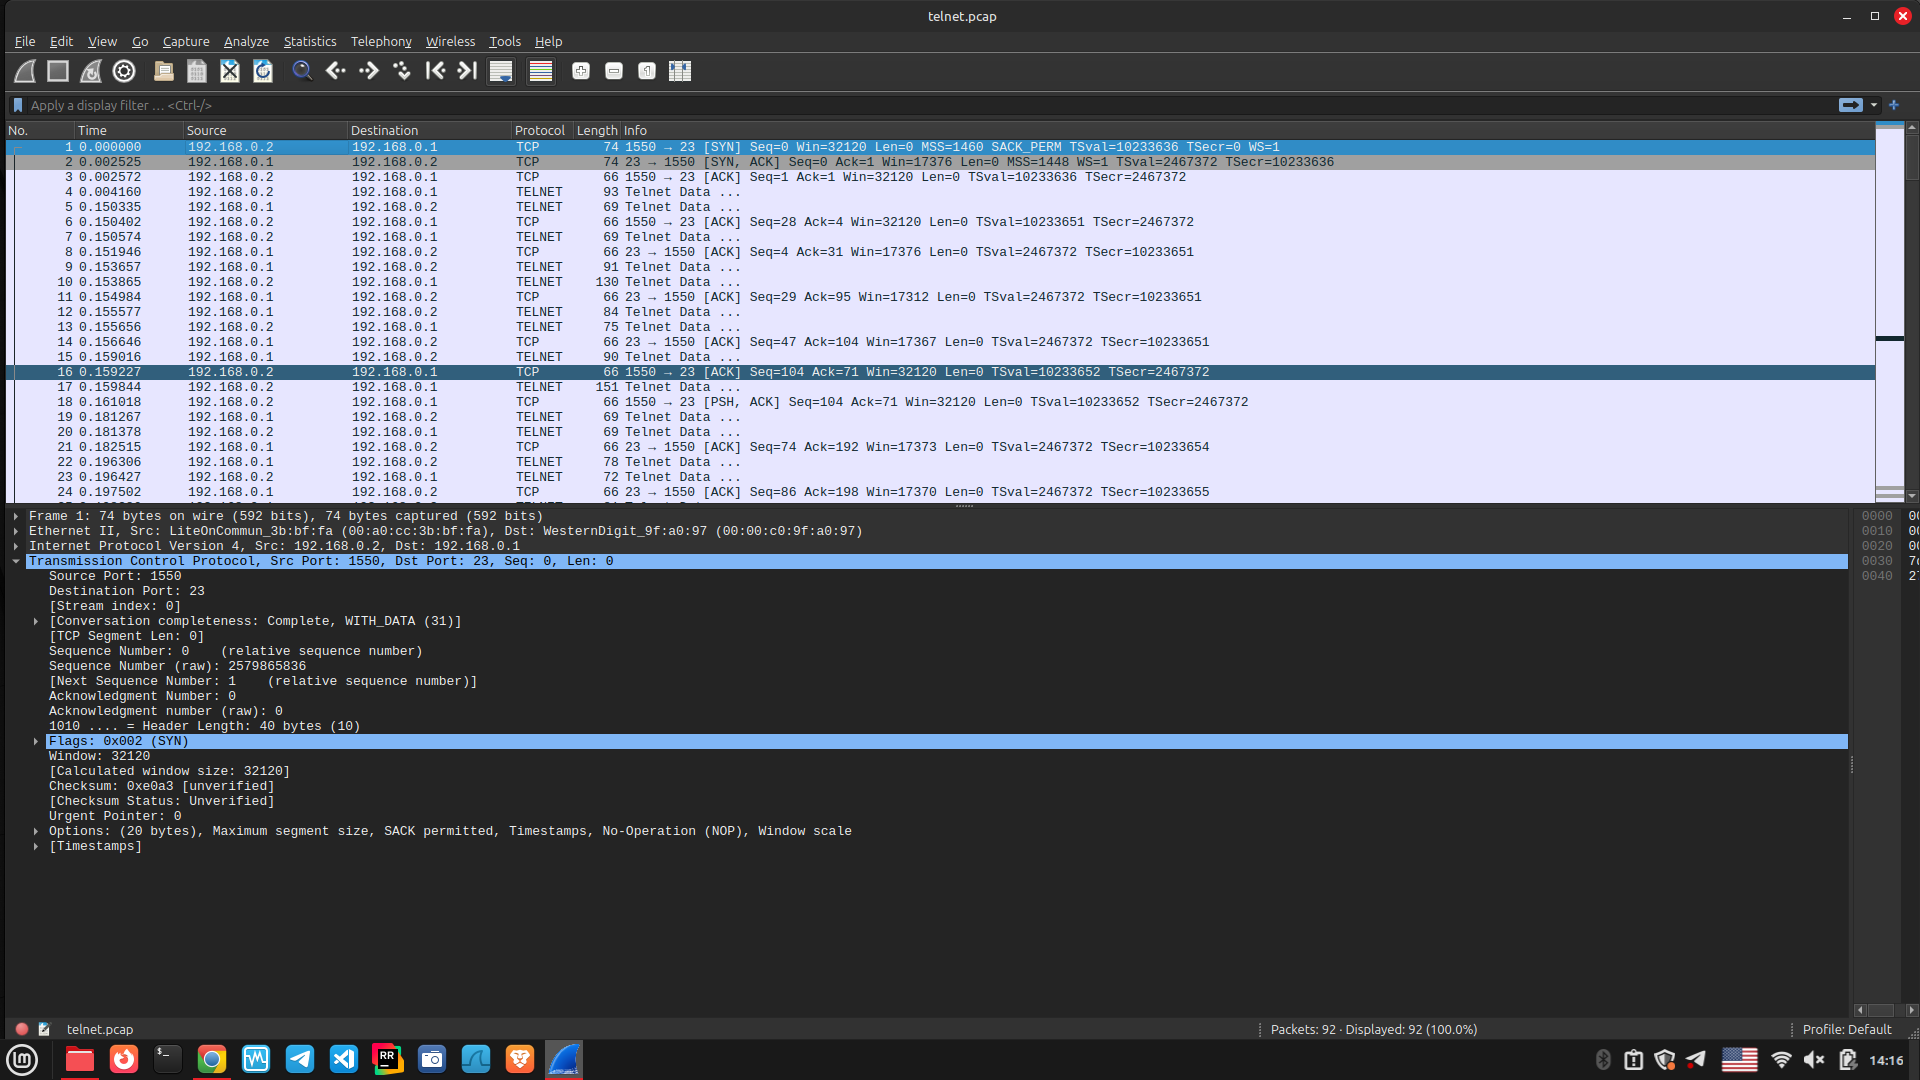
\includegraphics[width=0.4\textwidth]{report2-resources/telnet/telent3.png}
		\caption{بازیابی دنباله بسته‌ها و ساخت ارتباط TELNET از فایل داده شده.}
		\label{tel:3}
	\end{figure}
	\subsection{}
	در تصویر \ref{tel:4} دستورات اجرا شده توسط کلاینت قابل مشاهده است. دستورات با \& شروع شده و با رنگ قرمز می‌باشند.
	\begin{figure}[h]
		\centering
		\includegraphics[width=0.4\textwidth]{report2-resources/telnet/telent4.png}
		\caption{بازیابی دنباله بسته‌ها و ساخت ارتباط TELNET از فایل داده شده.}
		\label{tel:4}
	\end{figure}
	
	\section{DNS}
	\subsection{}
	ما تصمیم گرفتیم که برای اجرای دستور dig، از سایت \url{www.cloudflare.com} استفاده کنیم. همانطور که در تصویر 5 قابل مشاهده است، query برای resolver محلی با آدرس 192.168.126.56 ارسال شده است.
	\begin{figure}[h]
		\centering
		\includegraphics[width=0.4\textwidth]{report2-resources/telnet/telent4.png}
		\caption{درخواست و پاسخ سیستم با ریزالور محلی}
		\label{dns:1}
	\end{figure}
	
	
	\subsection{}
	

	
\end{document}
